\documentclass[a4paper,11pt]{article}
\usepackage[utf8]{inputenc}
\usepackage[paper=a4paper, hmargin=1.5cm, bottom=1.5cm, top=3.5cm]{geometry}
\usepackage[T1]{fontenc}
\usepackage[colorlinks=true, linkcolor=blue]{hyperref} %Links para el indice.
\usepackage{amsfonts}
\usepackage{verbatim}
\usepackage{listings}
\usepackage{caption}
\usepackage{subcaption}
\usepackage{graphicx}
\usepackage{wrapfig}
\usepackage[section]{placeins}
\usepackage{float}
%\usepackage{adjustbox}
\usepackage{amsmath}
\usepackage{blindtext}
\usepackage{sidecap}
\usepackage{color}

\captionsetup[subfigure]{labelformat=empty}

% \newcommand{\real}{\hbox{\bf R}}

\title{Protocolo ARP}

\begin{document}

\maketitle

\begin{center}
	Universidad de Buenos Aires - Departamento de Computaci\'on - FCEN
\end{center}

\vspace{2cm}
Integrantes:

\begin{itemize}
	\item Gallardo, Guillermo L.U.: 32/10 \verb+gagdiez.c@gmail.com+
	\item Fixman, Martin L.U.: 391/11 \verb+martinfixman@gmail.com+
	\item Matayoshi, Leandro L.U.: 79/11 \verb+leandro.matayoshi@gmail.com+
	\item Szyrej, Alexander L.U.: 642/11 \verb+alexander.szyrej@gmail.com+
		
\end{itemize}

\newpage

\tableofcontents

\newpage

\section{Introducción}

El protocolo ARP (\emph{Adress Resolution Protocol}) permite mapear direcciones IP a direcciones
físicas. Cuando un host desea comunicarse con otro dentro de una misma red local debe hacerlo
utilizando la \emph{MAC Adress} del mismo. Conociendo su dirección IP, puede \emph{brodcastear} un
paquete \emph{ARP who-has} pidiendo la \emph{MAC} asociada a dicha IP. De esta manera recibirá en
respuesta un paquete \emph{ARP-reply} por parte del host destino.
Para evitar una cantidad excesiva de broadcasts, cada nodo de la red mantiene su propia tabla de
mapeos que actualiza luego de cierto tiempo.

Cada paquete ARP incluye numerosos campos. Sin embargo, pondremos énfasis especialmente en los 
siguientes:
\begin{itemize}
    \item Operation: 1 (Request), 2 (Reply)
    \item Sender hardware adress: \emph{MAC} address source
    \item Sender protocol adress: \emph{IP} address source
    \item Target hardware adress: \emph{MAC} address dest
    \item Target protocol adress: \emph{IP} address dest
\end{itemize}

El objetivo de este trabajo práctico es analizar el flujo de paquetes \emph{who-has} en distintas
redes no contraladas. Luego, en base a la informaci\'on recopilada, analizaremos el rol que juega
cada dispositivo dentro de la red. De esta manera podemos corroborar de manera empírica el 
comportamiento establecido por el protocolo \emph{ARP} para el envío de paquetes en una red local.  


\section{Desarrollo}

\section{Desarrollo}

El primer paso en este trabajo fue implementar un script en \emph{python} 
para escuchar pasivamente paquetes dentro de la red local. Para esto capturamos
todos los paquetes que circulan utilizando la librería Scapy, y nos quedamos 
solo con los ARP de tipo \emph{who-has}. Luego, contamos cuantas veces aparece
una direcci\'on en cada campo, as\'i como tambi\'en la interacci\'on entre
todos los pares de ip. Terminamos ordenando esta información según la
cantidad de paquetes, de mayor a menor.

Con estas observaciones nos proponemos a calcular la entropia tomando dos 
modelos distintos de fuente: en \textbf{$S_{src}$} los símbolos son las
direcciones IP que aparecen en el campo SRC; en \textbf{$S_{dst}$} son las
direcciones IP que aparecen en el campo DST.

En relación a esto tenemos una mejor base para realizar un análisis del estado de 
la red al momento de las mediciones, y podemos analizar estadísticamente qué IPs 
son más relevantes o significativas en la LAN utilizando la información del símbolo 
con respecto a la entropía de la fuente correspondiente.


En la próxima sección podrán verse los datos obtenidos y el análisis de los mismos
para las distintas redes en las cuales fueron realizadas las capturas: 
\textcolor{red}{Entrepiso DC} (\textbf{2634} paquetes), \textcolor{red}{Fibertel Zone} de Starbucks (\textbf{500} paquetes),
\textcolor{red}{Casa de Familia} (\textbf{515} paquetes) y \textcolor{red}{Empresa} (\textbf{400} paquetes).





\clearpage

\section{Resultados y análisis}

\section{Resultados y An\'alisis}

\subsection{Casa Familia}

\FloatBarrier

\FloatBarrier

\begin{figure}[!h]
	\begin{center}
		  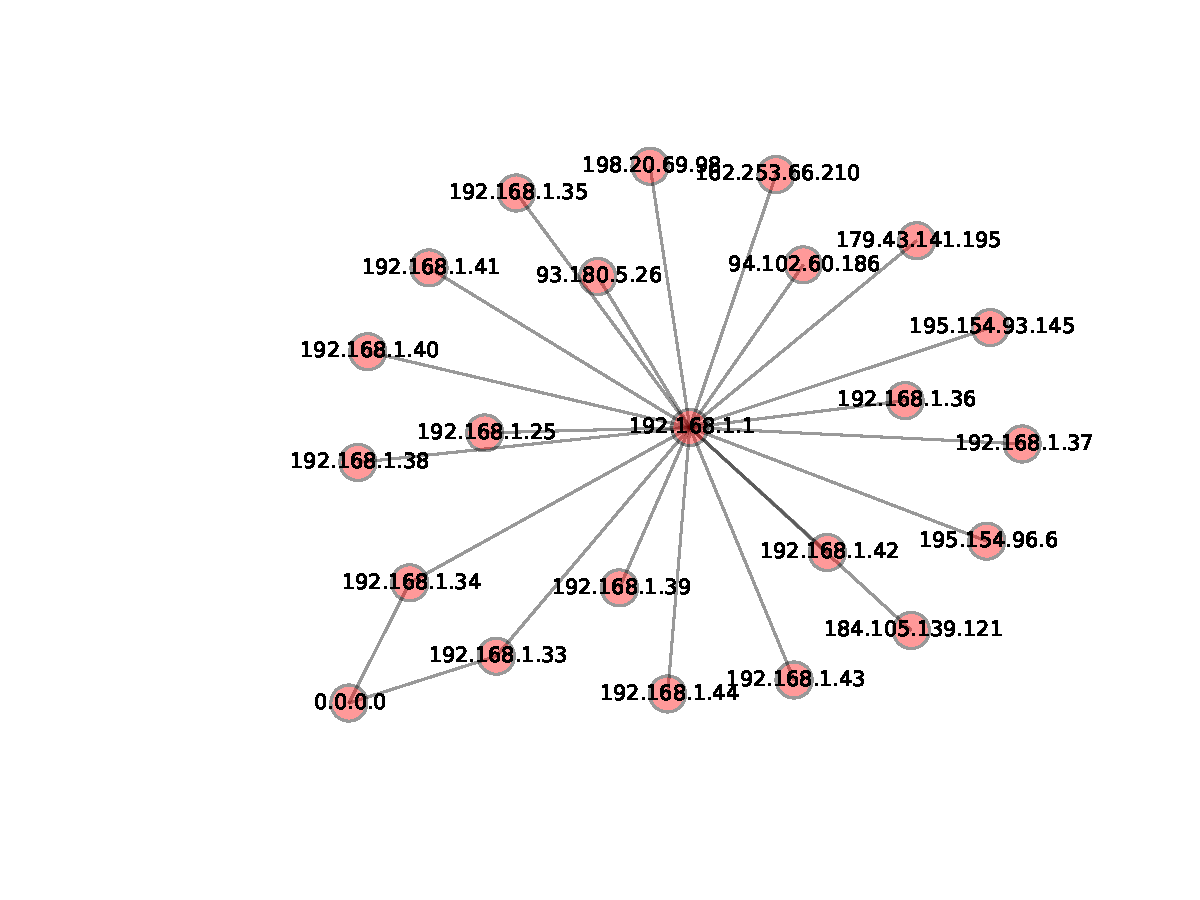
\includegraphics[scale=0.75]{resultados/casa/conectividadNX.pdf}
		  \caption{Grafo de conectividad la red casa}
		  \label{fig:contra1}
	\end{center}
\end{figure}
	
\FloatBarrier

En el caso de la casa familiar sabemos que la direcci\'on del router
es 192.168.1.1 y que 192.168.1.35 pertenece al dispositivo que m\'as tiempo estuvo
prendido, el mismo es una notebook. Podemos apreciar que la ip del
router es de las que aparece con mayor frecuencia en los campos SRC (fig \emph{a}) 
o DST (fig \emph{b}), mientras que la notebook solo aparece un alto n\'umero de 
veces en DST. 

En la \emph{Figura 1} podemos ver que la red local se puede representar como 
un grafo en forma de estrella, el mismo tiene al router como centro. 

La entrop\'ia fue: $1.68$ para el modelo $SRC$ y $2.67$ para el modelo DST.
Cabe destacar que aunque no est\'a reflejado en los gr\'aficos, sucedi\'o algo interesante, 
aparecieron paquetes ARP con direcciones que no pertenecian a la red local.

~
\FloatBarrier

\begin{figure}[!h]
	\begin{center}
		  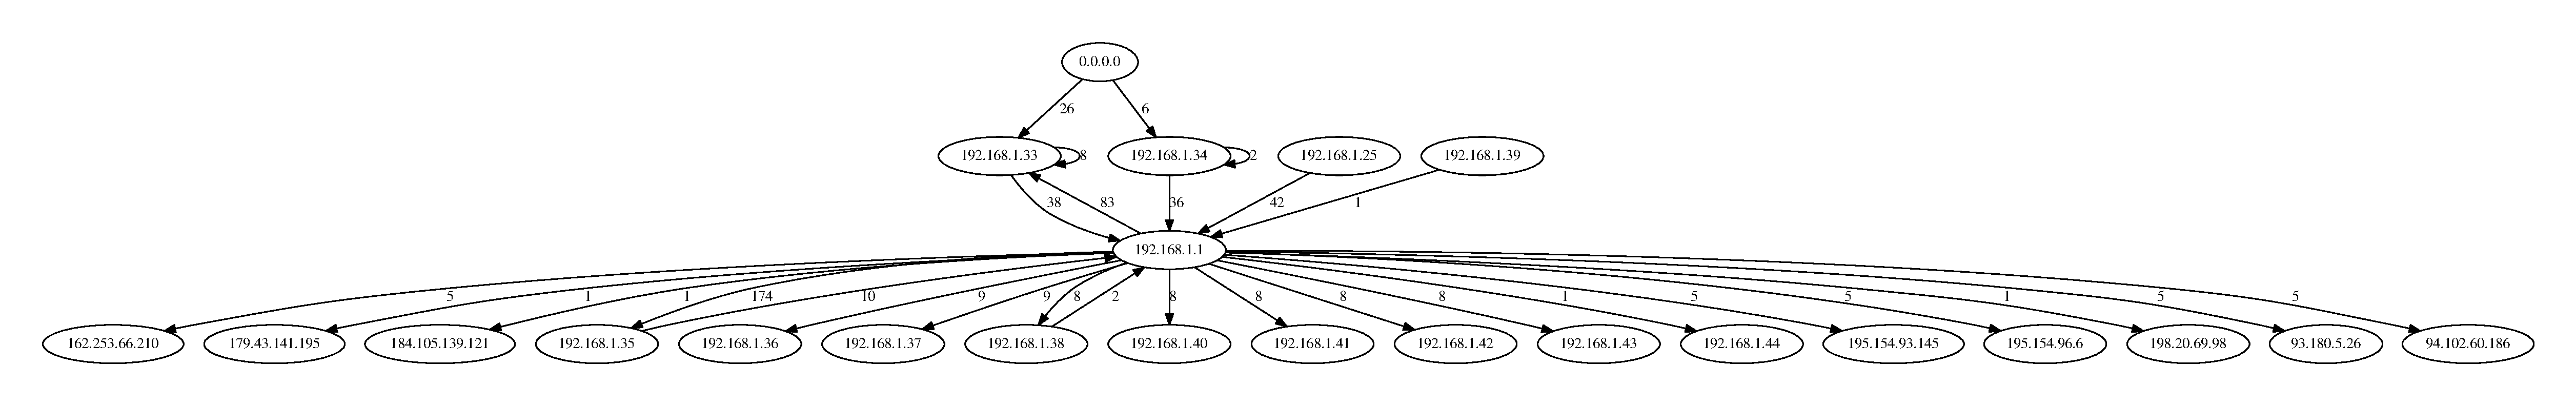
\includegraphics[scale=0.23]{resultados/casa/conectividad.pdf}
		  \caption{Grafo con pesos en las aristas de la red Casa}
		  \label{fig:contra1}
	\end{center}
\end{figure}

\FloatBarrier

~

\begin{figure}[H]
	\center
	\begin{subfigure}{0.4\textwidth}
		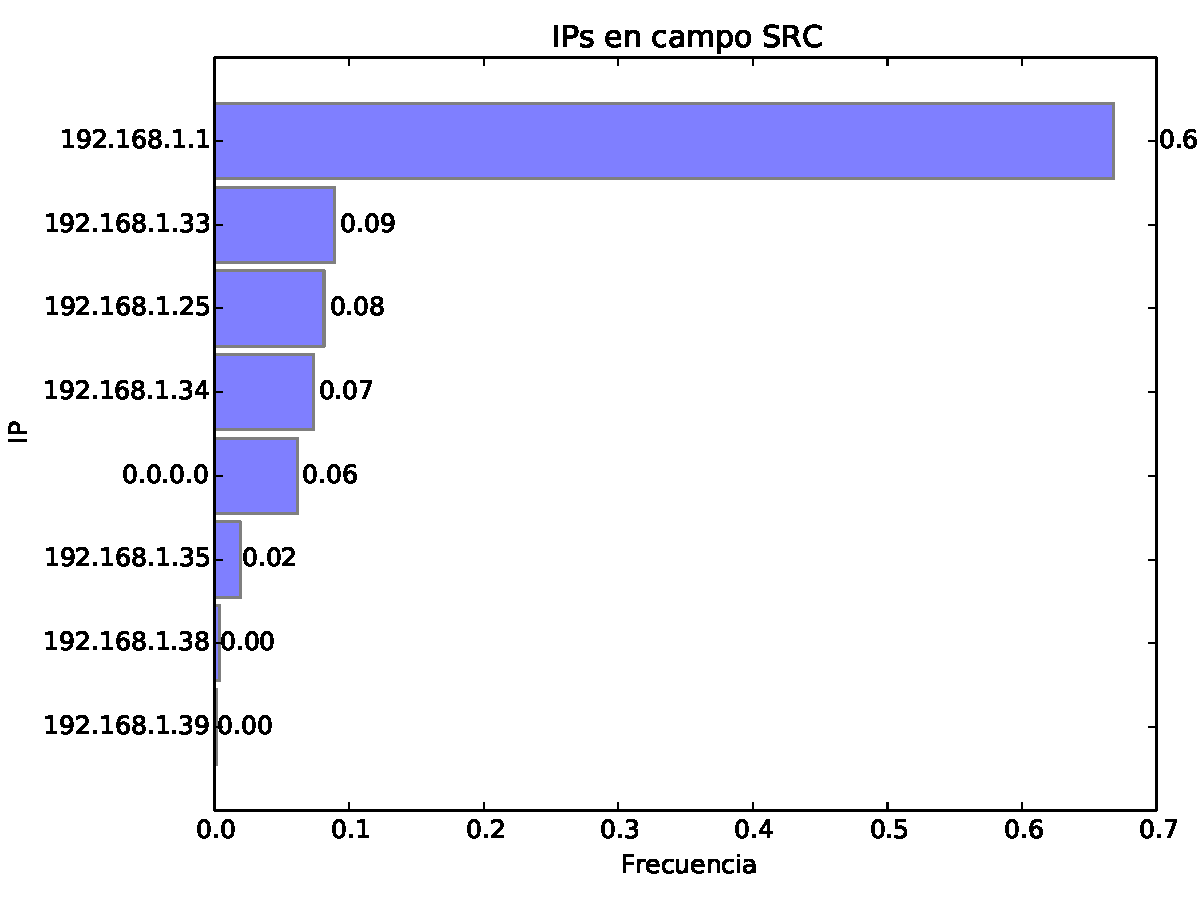
\includegraphics[width=1.0\textwidth]{resultados/casa/ipsSrc_1_6805902069.pdf}
		\caption{Estimaci\'on de la probabilidad de cada s\'imbolo en modelo SRC}
	\end{subfigure}
	~
	\begin{subfigure}{0.4\textwidth}
		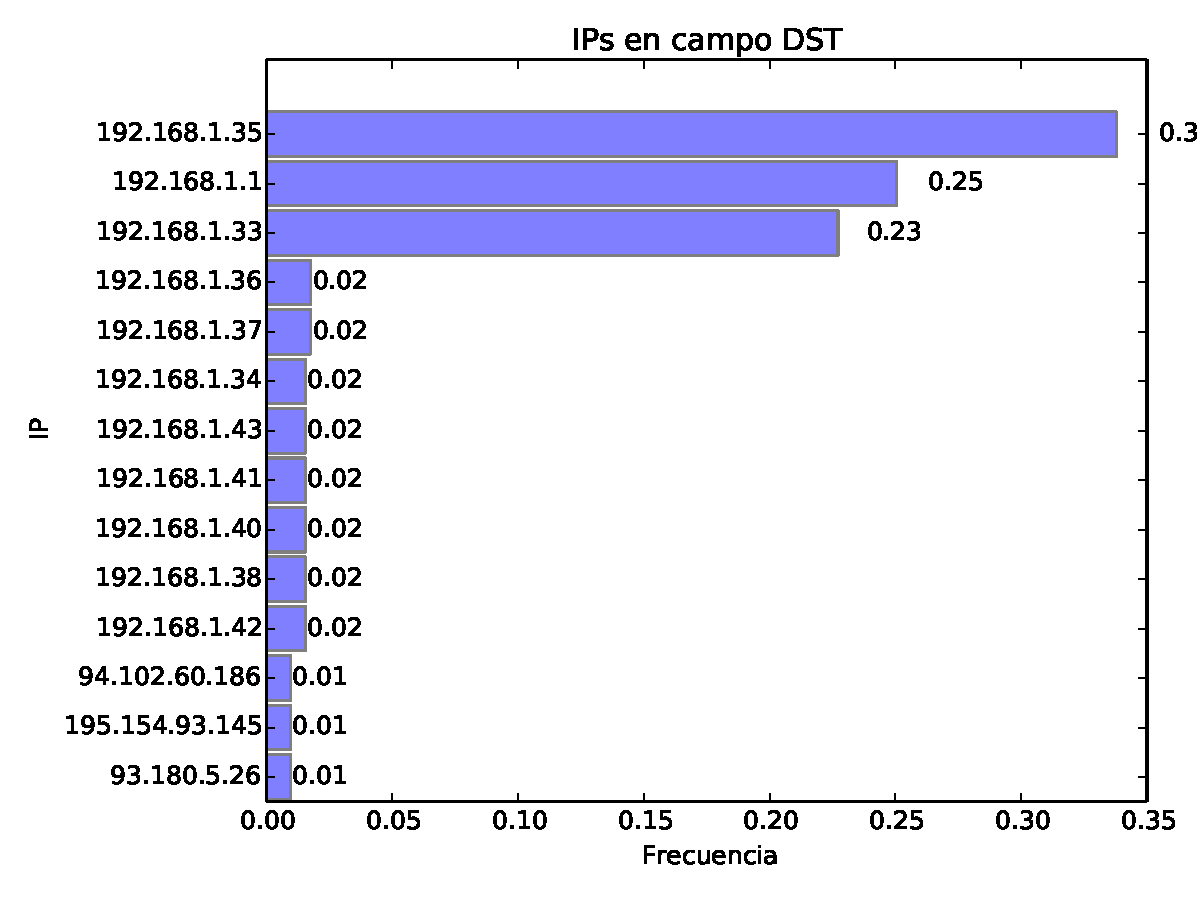
\includegraphics[width=1.0\textwidth]{resultados/casa/ipsDst_2_67355481854.pdf}
		\caption{Estimaci\'on de la probabilidad de cada s\'imbolo en modelo DST}
	\end{subfigure}
\end{figure}


\subsection{Empresa}

Nuevamete, en esta red teníamos conocimiento de quien era el router y las computadoras mas 
importantes. 
Lo primero que notamos en este caso fue que la topología del grafo de la red (\emph{Figuras 4 y 5})
no coincide con la de una estrella. Es posible observar una interacción mucho mayor 
entre distintos pares hosts, y no únicamente entre cada uno de estos y el router.

\subsection{Starbucks}

%\begin{wrapfigure}{R}{0.4\textwidth}
%\vspace{-20pt}
%\hspace{-35pt}
%\centering
%   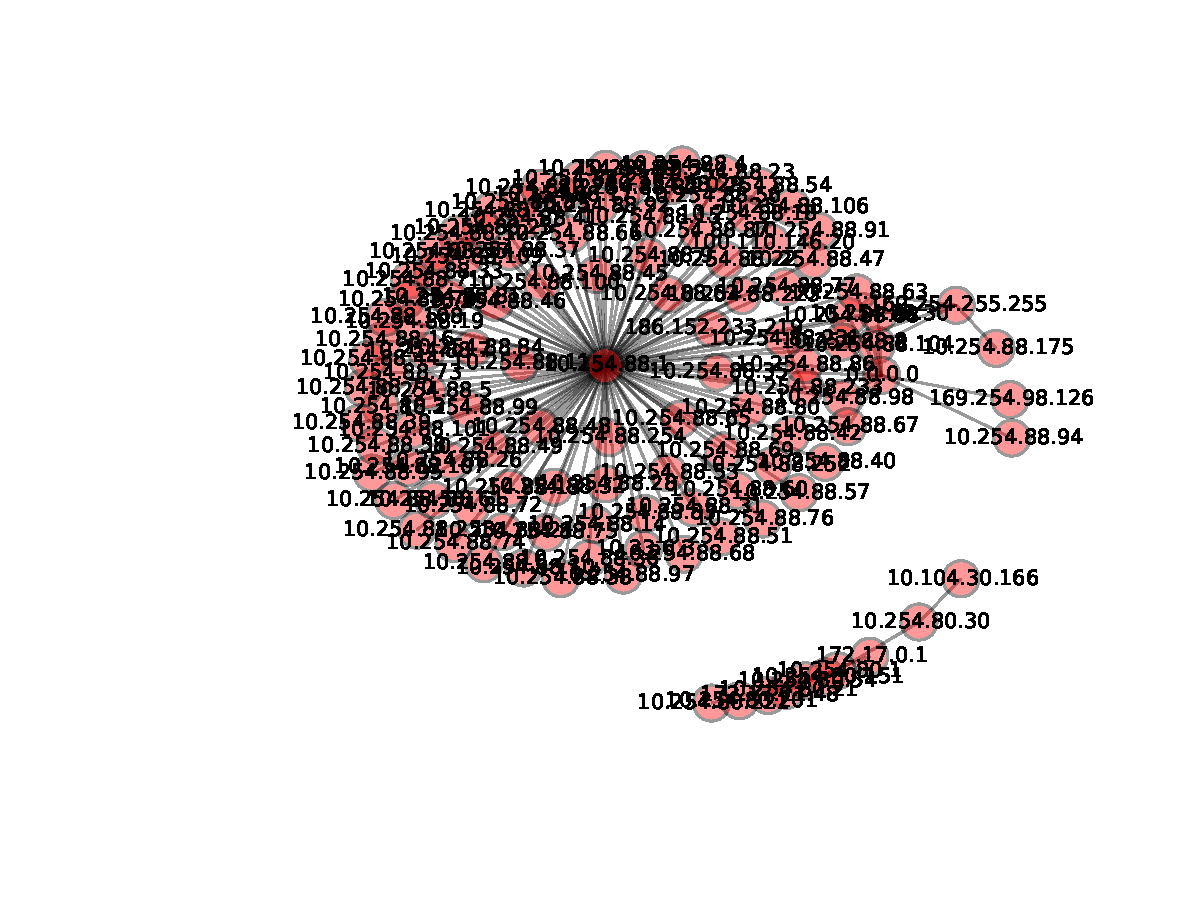
\includegraphics[width=0.4\textwidth]{resultados/starbucks/conectividadNX.pdf}
%\vspace{-30pt}
%   \caption{Grafo de la red}
%\end{wrapfigure}

Para el caso de la red abierta disponible en Starbucks, podemos ver en el 
grafo simple una notoria centralizaci\'on de paquetes hacia/desde la direcci\'on
10.254.88.1, la cual a su vez posee una alta frecuencia de aparici\'on en ambos
modelos. Esto ser\'ia el comportamiento esperado del router de la red
10.254.88.0/24. Asumimos que \'esta es la direcci\'on de la red puesto que 
la mayor\'ia de las IPs de los paquetes capturados difieren en el \'ultimo octeto.
Por otro lado, podemos ver que la segunda direcci\'on con mayor frecuencia en DST
fue 10.254.80.1, seguida por 10.254.88.8. Suponemos que $88.8$ es la pc del lugar
dada la ip baja, y la cantidad de apariciones. Por otro lado, no sabemos que es
$80.1ç$ dado que parece formar una red aparte de la sniffeada.

La entrop\'ia fue: $4.61$ para el modelo $SRC$ y $3.76$ para el modelo
DST.


Nuevamente entre los paquetes capturados volvieron a aparecer direcciones que
no parecieran pertenecer a la red local, resultando sumamente interesante el caso
de 10.254.80.1


\begin{figure}[H]
	\center
	\begin{subfigure}{0.4\textwidth}
		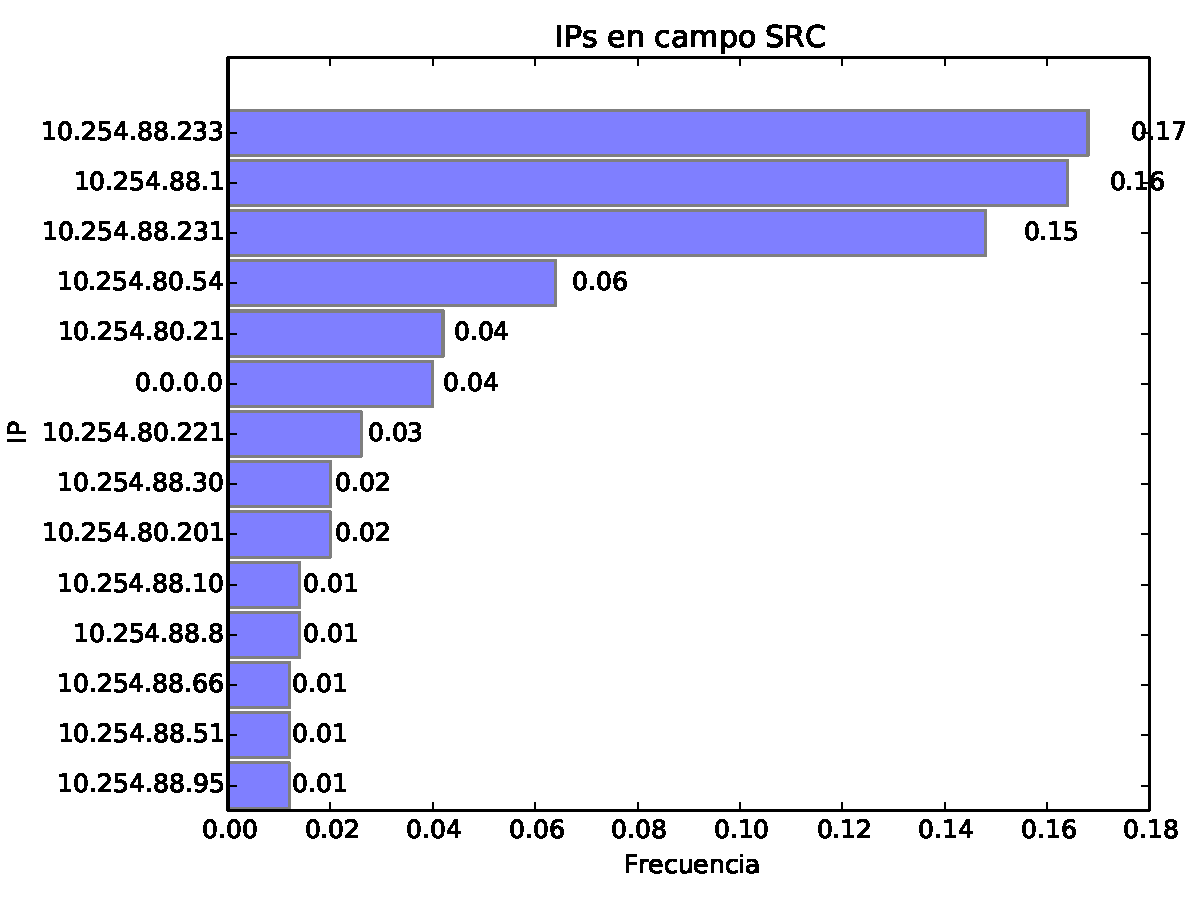
\includegraphics[width=1.0\textwidth]{resultados/starbucks/ipsSrc_4_6187931499.pdf}
		\caption{Estimaci\'on de la probabilidad de cada s\'imbolo en modelo SRC}
	\end{subfigure}
	~
	\begin{subfigure}{0.4\textwidth}
		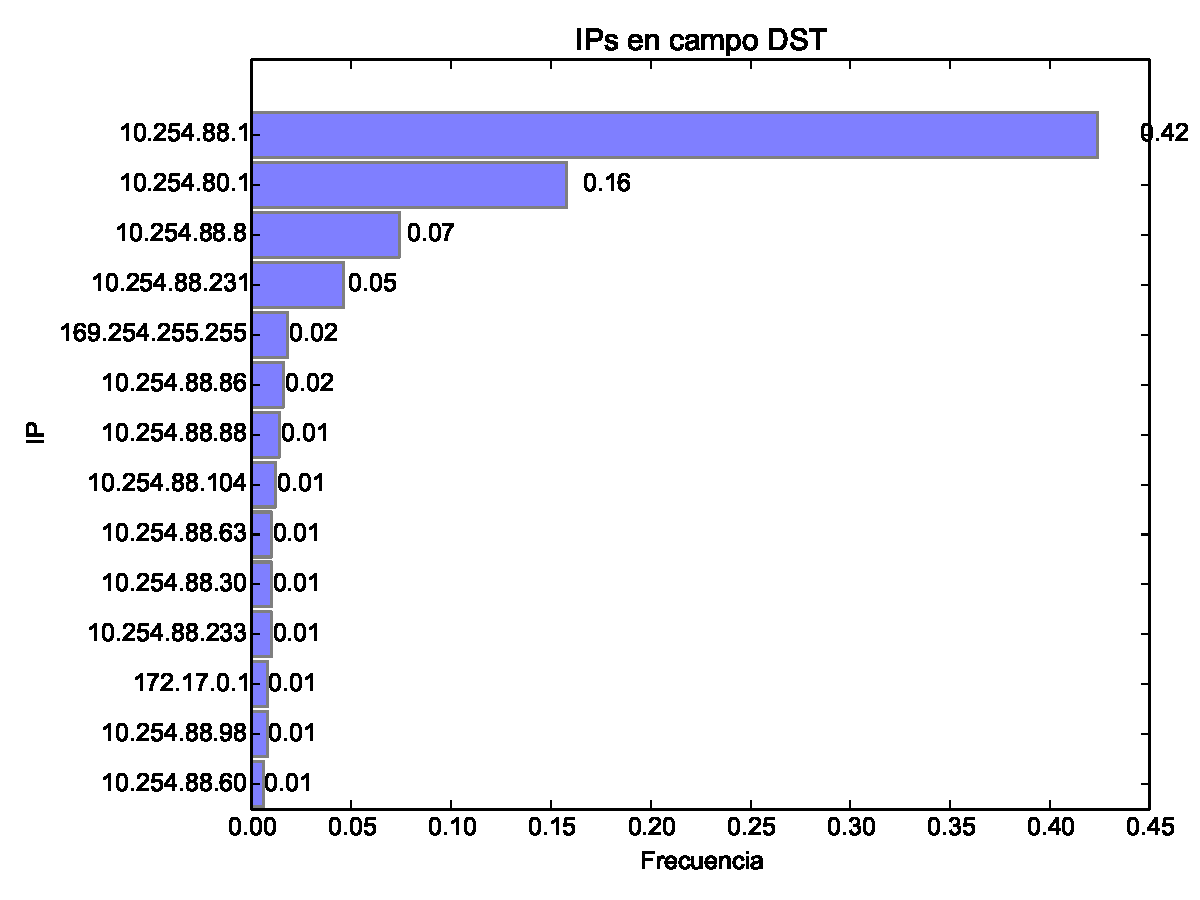
\includegraphics[width=1.0\textwidth]{resultados/starbucks/ipsDst_3_76848714287.pdf}
		\caption{Estimaci\'on de la probabilidad de cada s\'imbolo en modelo DST}
	\end{subfigure}
\end{figure}

\FloatBarrier

~

\begin{figure}[H]
	\center
	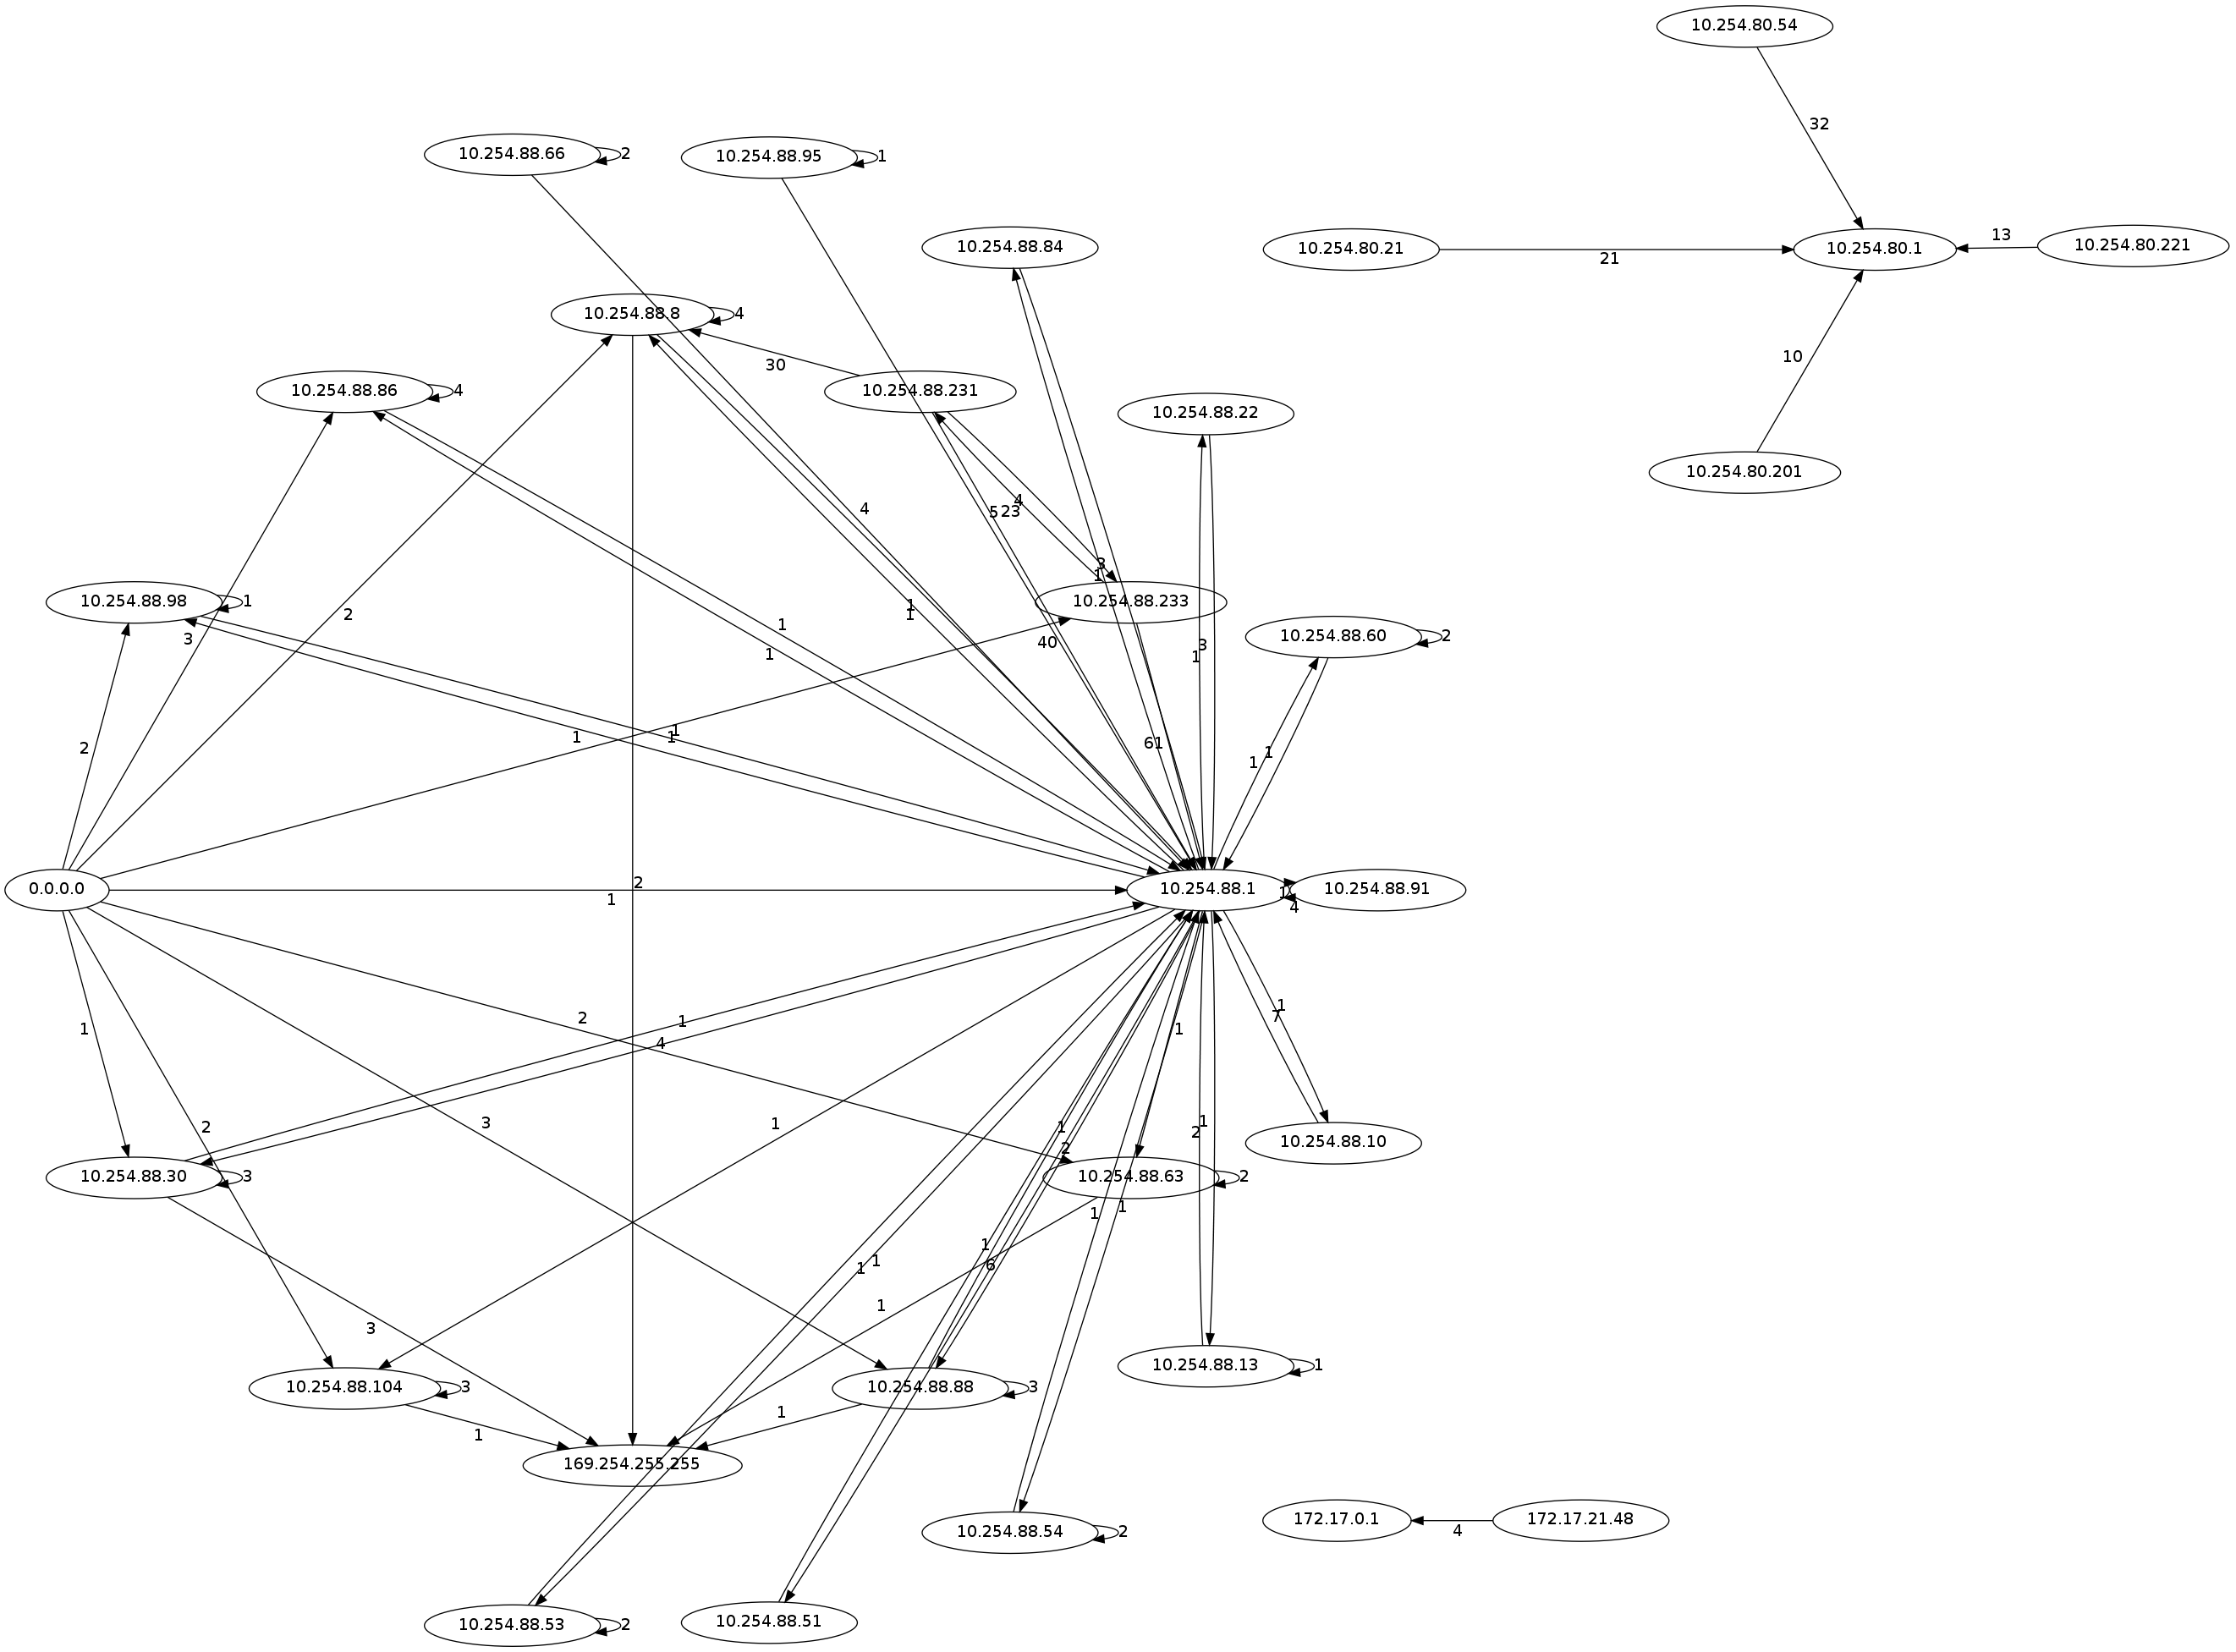
\includegraphics[width=0.9\textwidth]{resultados/starbucks/starbucks.png}
	\caption{Grafo con pesos en las aristas de la red Starbucks}
\end{figure}

~

\FloatBarrier

\begin{figure}[!h]
	\begin{center}
		  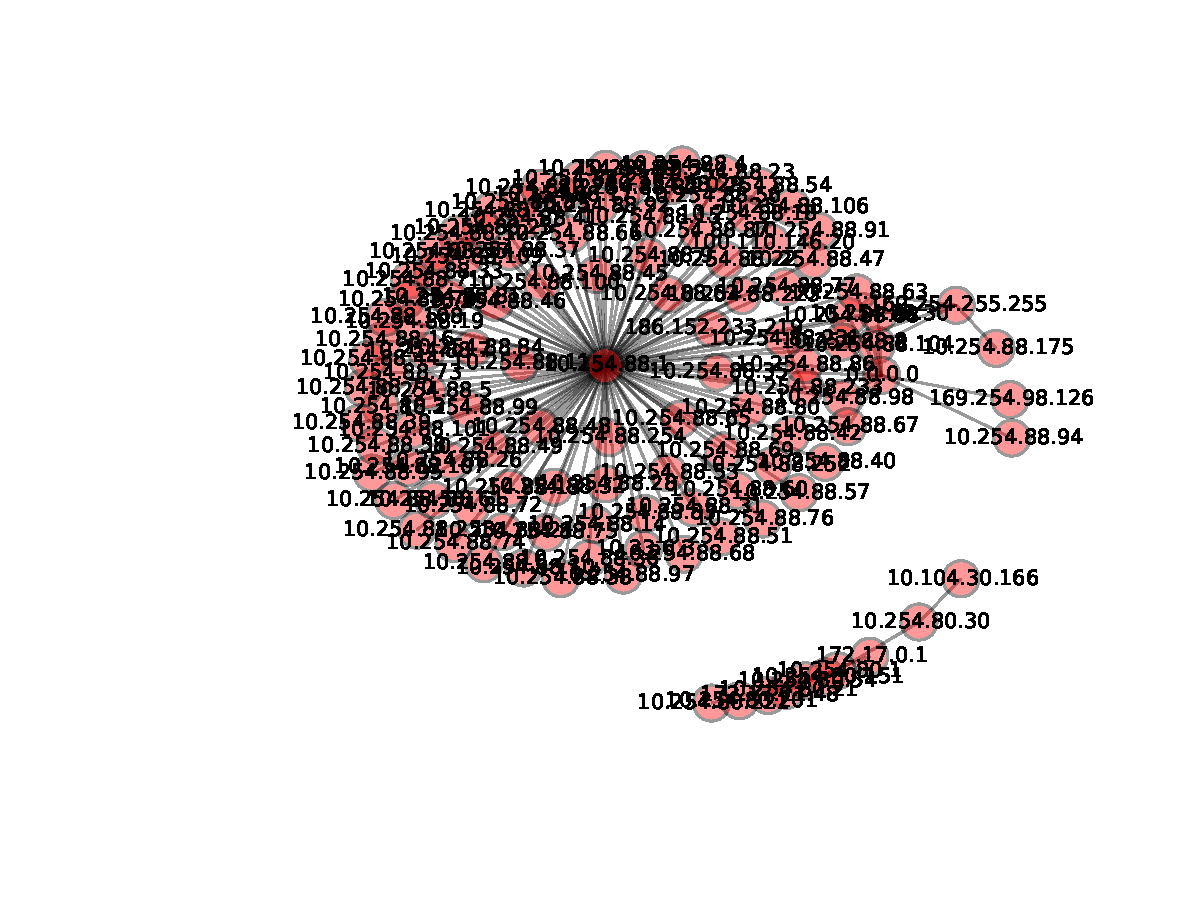
\includegraphics[scale=1.00]{resultados/starbucks/conectividadNX.pdf}
		  \caption{Grafo de conectividad la red Starbucks}
		  \label{fig:contra1}
	\end{center}
\end{figure}
	

\FloatBarrier

\subsection{Empresa}


En este caso la topología del grafo de la red no coincide con la de una estrella. Es posible observar una interacción mucho mayor entre distintos pares hosts, y no únicamente
entre cada uno de estos y el router.

\begin{figure}[H]
	\center
	\begin{subfigure}{0.4\textwidth}
		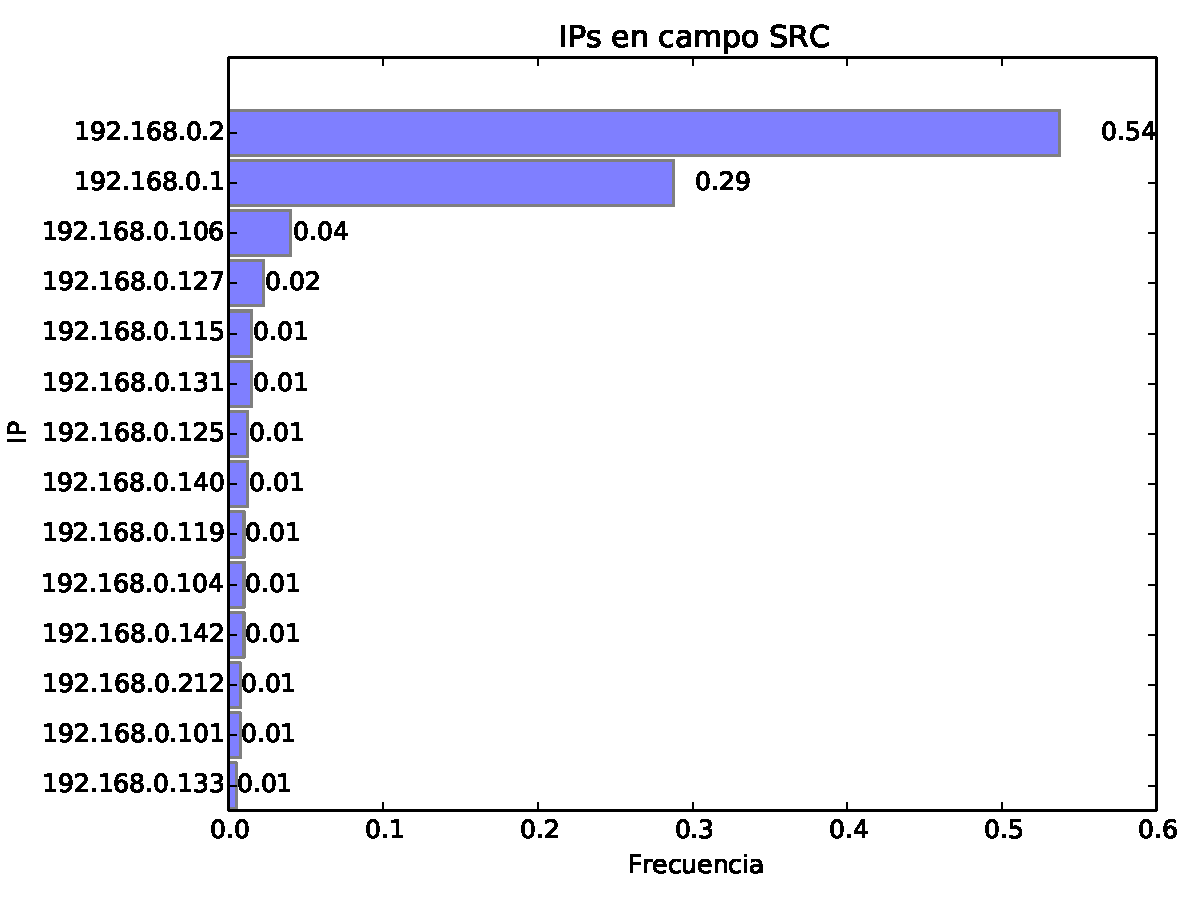
\includegraphics[width=1.0\textwidth]{resultados/empresa/ipsSrc_2_05542931604.pdf}
		\caption{Estimaci\'on de la probabilidad de cada s\'imbolo en modelo SRC}
	\end{subfigure}
	~
	\begin{subfigure}{0.4\textwidth}
		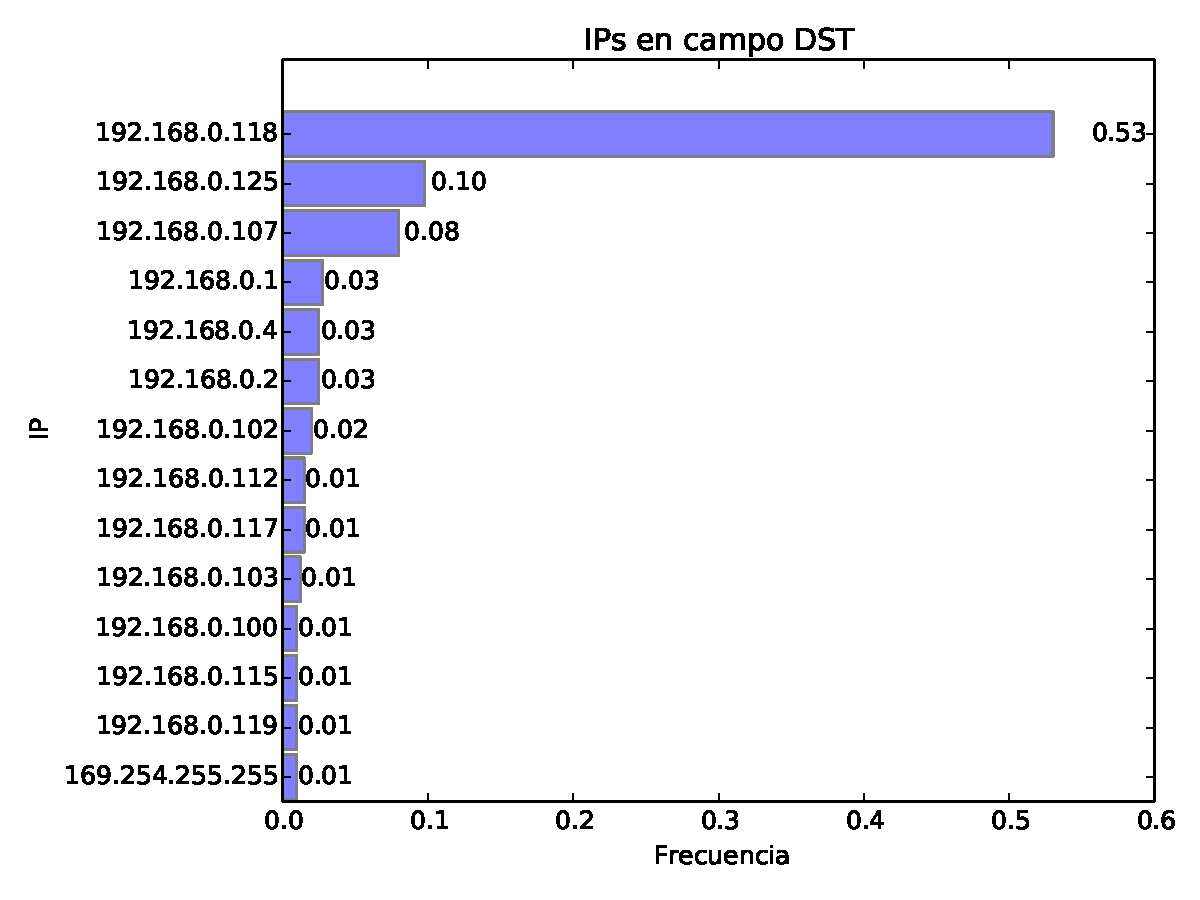
\includegraphics[width=1.0\textwidth]{resultados/empresa/ipsDst_2_99926622579.pdf}
		\caption{Estimaci\'on de la probabilidad de cada s\'imbolo en modelo DST}
	\end{subfigure}
\end{figure}

En el gráfico de barras del modelo SRC el router juega un papel relevante ya que es el segundo
símbolo con mayor cantidad de emisión de paquetes. Es interesante mencionar que el 
nodo con mayor cantidad de paquetes enviados, cuya ip es 192.168.0.2, corresponde a un servidor apache.
El resto de los nodos que aparecen en el gráfico corresponden a notebooks
y celulares conectados a la red.

~

\begin{figure}[!h]
	\begin{center}
		  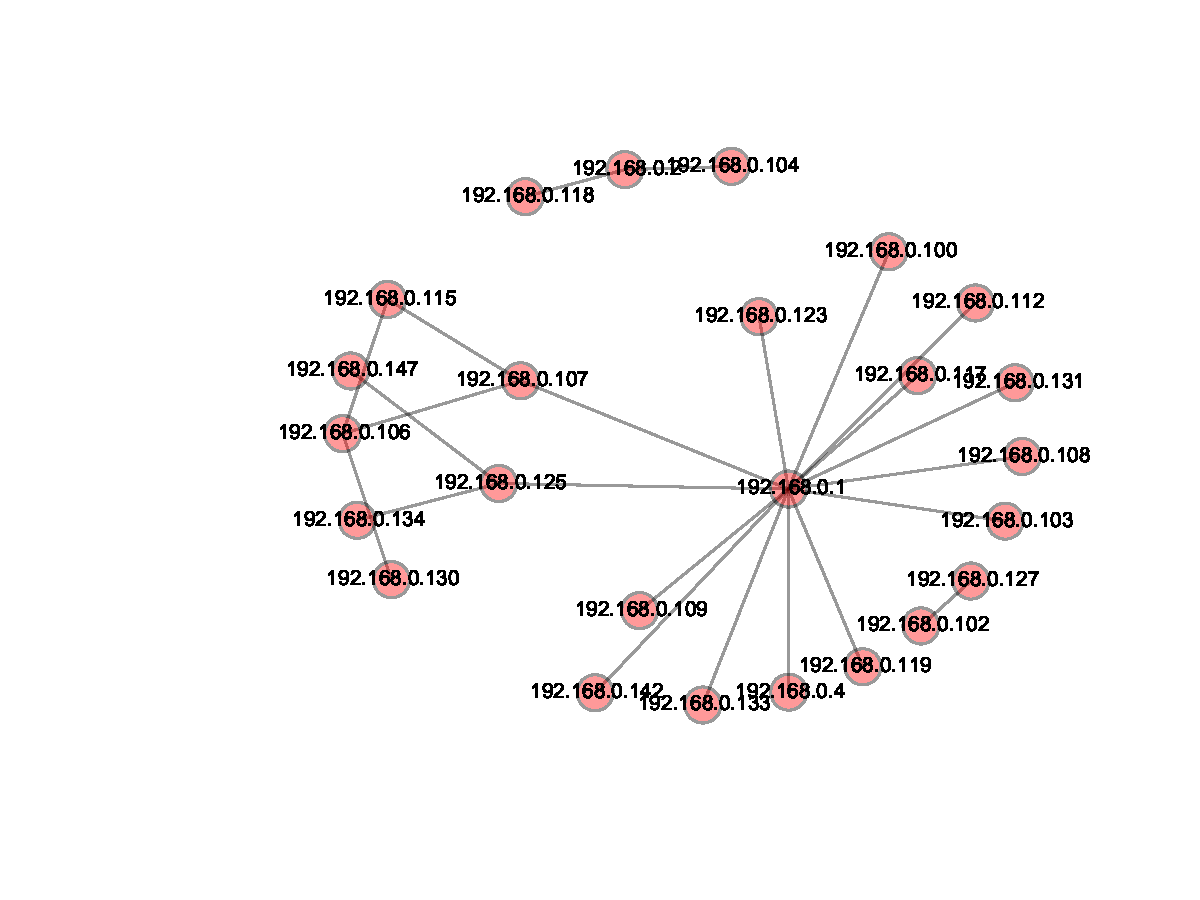
\includegraphics[scale=0.75]{resultados/empresa/conectividadNX.pdf}
		  \caption{Topología de la red empresa}
		  \label{fig:contra1}
	\end{center}
\end{figure}

~

En el gráfico de barras del modelo DST es en donde se nota la mayor cantidad de diferencias. 
El router no se corresponde con ninguno de los 3 nodos con mayor cantidad de paquetes
recibidos:

\begin{itemize}
    \item 192.168.0.118 corresponde a una notebook
    \item 192.168.0.125 corresponde a un servidor apache
    \item 192.168.0.107 corresponde a un servidor apache
\end{itemize}

Recién aparece en la cuarta posición, con una cantidad de paquetes recibidos considerablemente
menor a los primeros. En esta red en particular los dispositivos se envían paquetes
who-has entre ellos en mayor medida, y hacia los servidores en vez de hacia el router.

El valor de la entropía para el modelo SRC es $2.05$. El valor de la entropía para 
el modelo DST es $2.99$


~

Los gráficos de barra muestran que el router ha perdido preponderancia respecto a la emisión
y recepción de paquetes en comparación con otros nodos distinguidos.

\begin{figure}[H]
	\center
	\includegraphics[scale = 0.18]{resultados/empresa/conectividad.pdf}
	\caption{Grafo con pesos es las aristas de la red Empresa}
\end{figure}

~

\subsection{Starbucks}

Para el caso de la red abierta disponible en Starbucks, podemos ver en la 
\emph{Figura 7} una notoria centralizaci\'on de paquetes hacia/desde la direcci\'on
10.254.88.1, la cual a su vez posee una alta frecuencia de aparici\'on en ambos
modelos. Esto ser\'ia el comportamiento esperado del router de la red
10.254.88.0/24. Asumimos que \'esta es la direcci\'on de la red puesto que 
la mayor\'ia de las IPs de los paquetes capturados difieren en el \'ultimo octeto.
Por otro lado, podemos ver que la segunda direcci\'on con mayor frecuencia en DST
fue 10.254.80.1, seguida por 10.254.88.8. Suponemos que $88.8$ es la pc del lugar
dada la ip baja, y la cantidad de apariciones. Por otro lado, no sabemos que es
$80.1$ dado que parece formar una red aparte de la sniffeada.

La entrop\'ia fue: $4.61$ para el modelo $SRC$ y $3.76$ para el modelo
DST.

Nuevamente entre los paquetes capturados volvieron a aparecer direcciones que
no parecieran pertenecer a la red local, resultando sumamente interesante el caso
de 10.254.80.1


\begin{figure}[H]
	\center
	\begin{subfigure}{0.4\textwidth}
		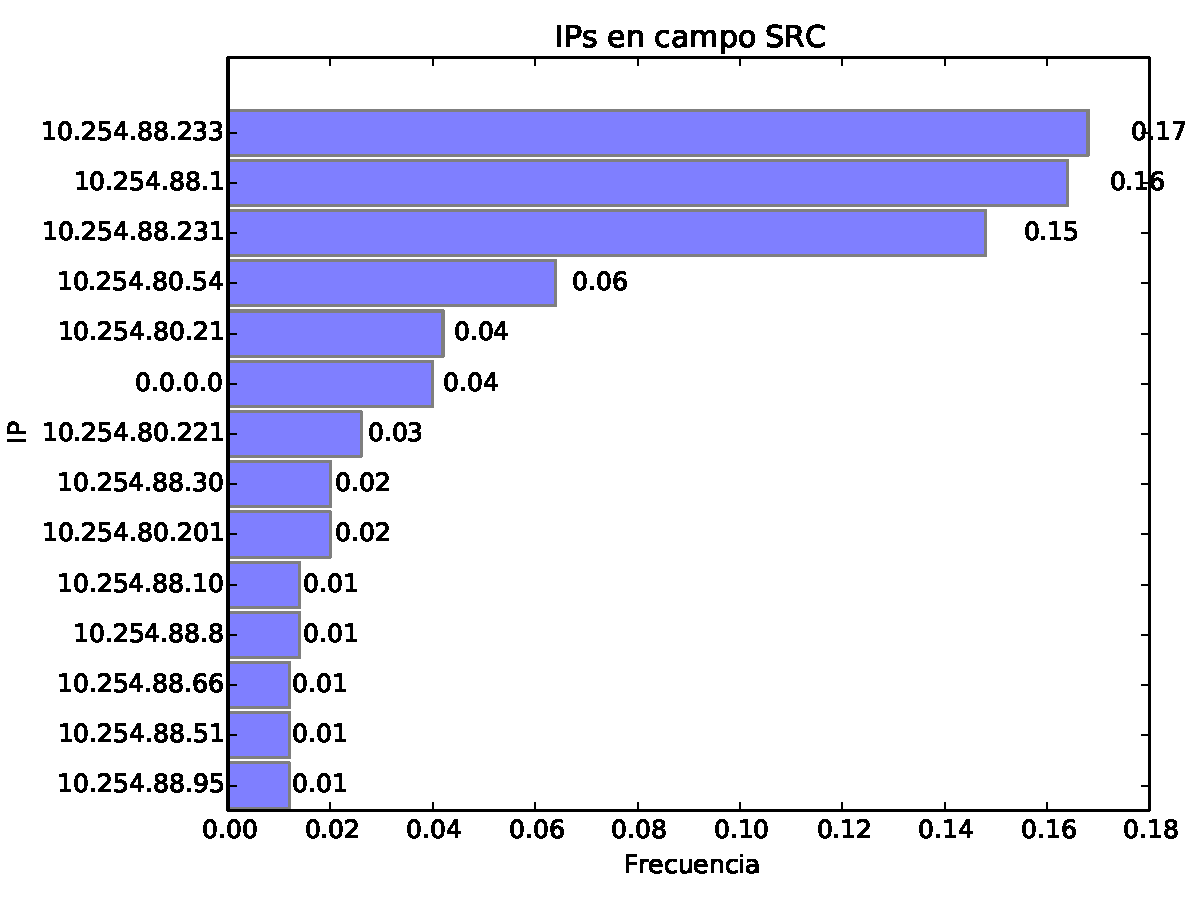
\includegraphics[width=1.0\textwidth]{resultados/starbucks/ipsSrc_4_6187931499.pdf}
		\caption{Estimaci\'on de la probabilidad de cada s\'imbolo en modelo SRC}
	\end{subfigure}
	~
	\begin{subfigure}{0.4\textwidth}
		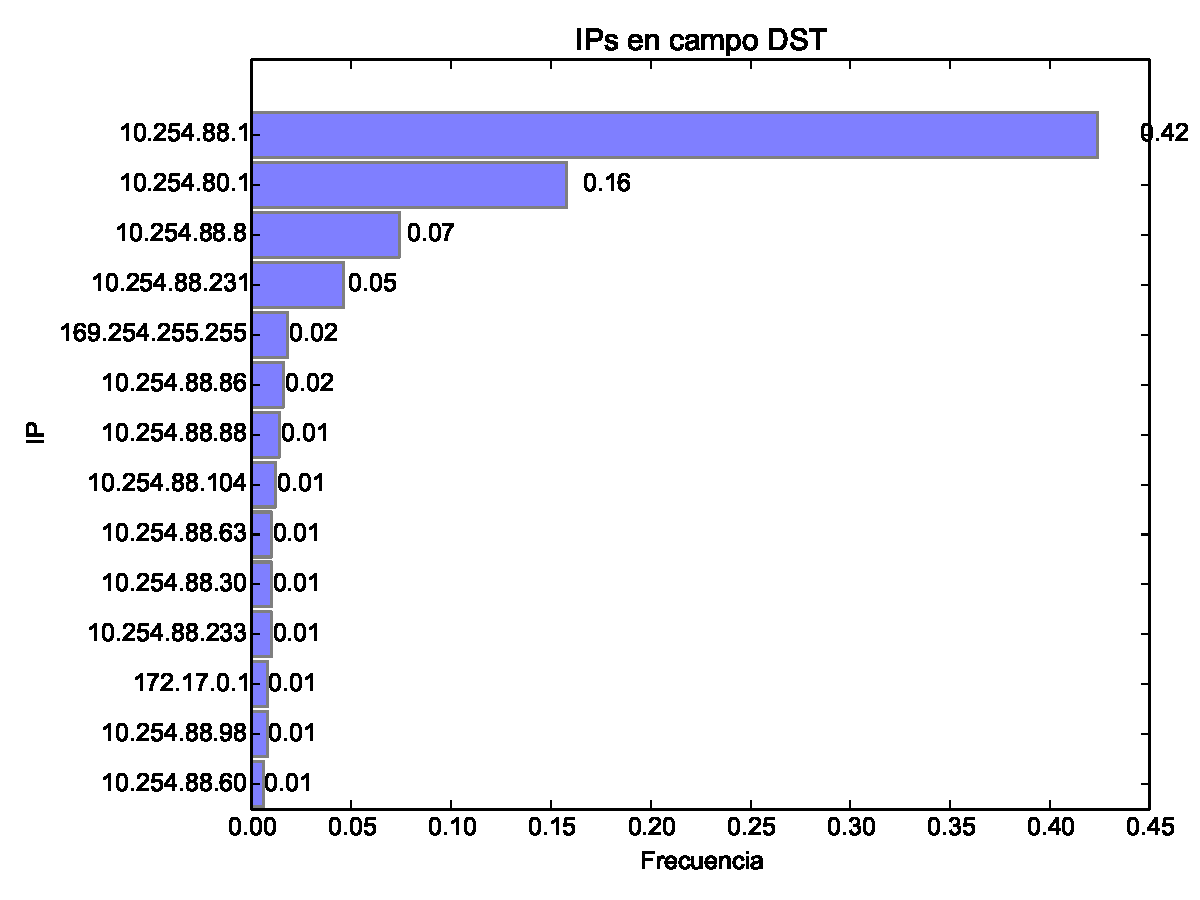
\includegraphics[width=1.0\textwidth]{resultados/starbucks/ipsDst_3_76848714287.pdf}
		\caption{Estimaci\'on de la probabilidad de cada s\'imbolo en modelo DST}
	\end{subfigure}
\end{figure}

~

\begin{figure}[H]
	\center
%	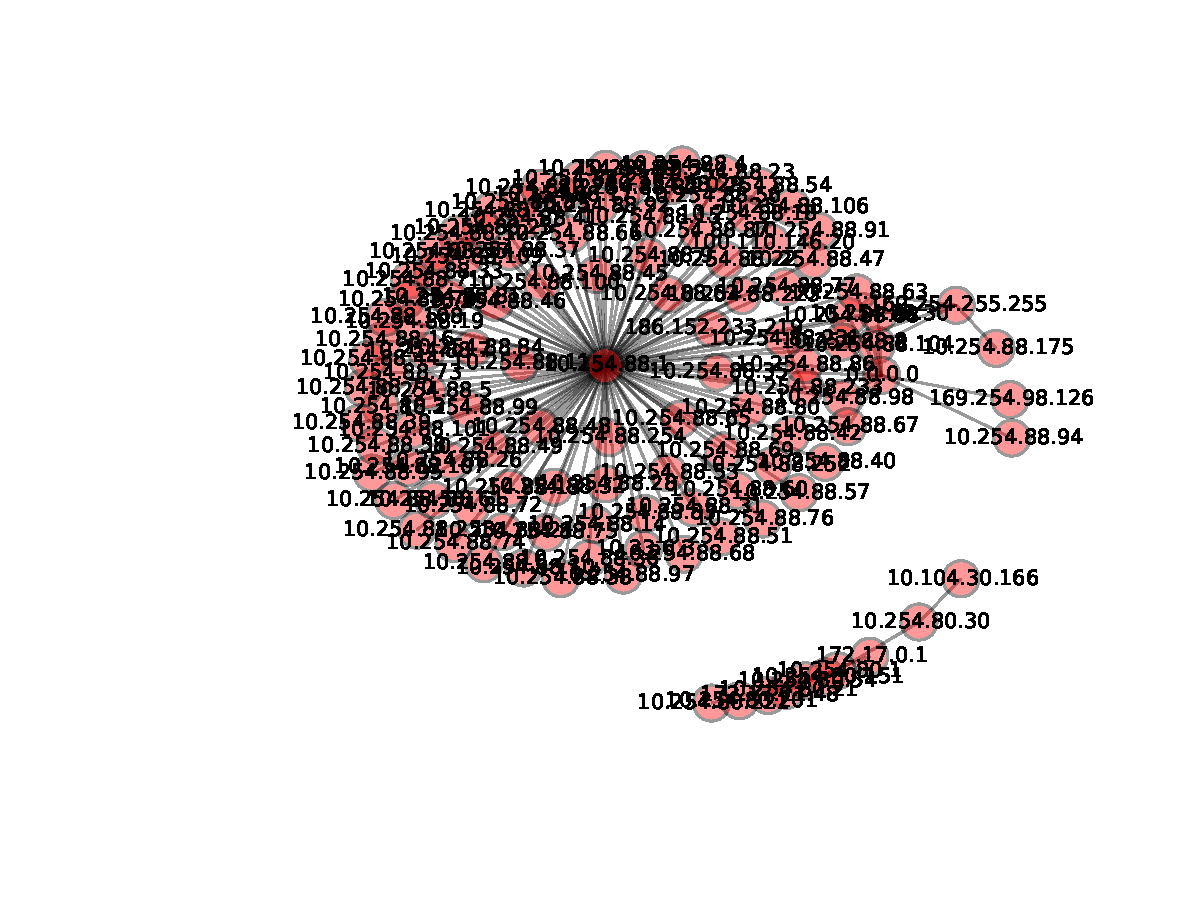
\includegraphics[width=1\textwidth]{resultados/starbucks/conectividadNX.pdf}
	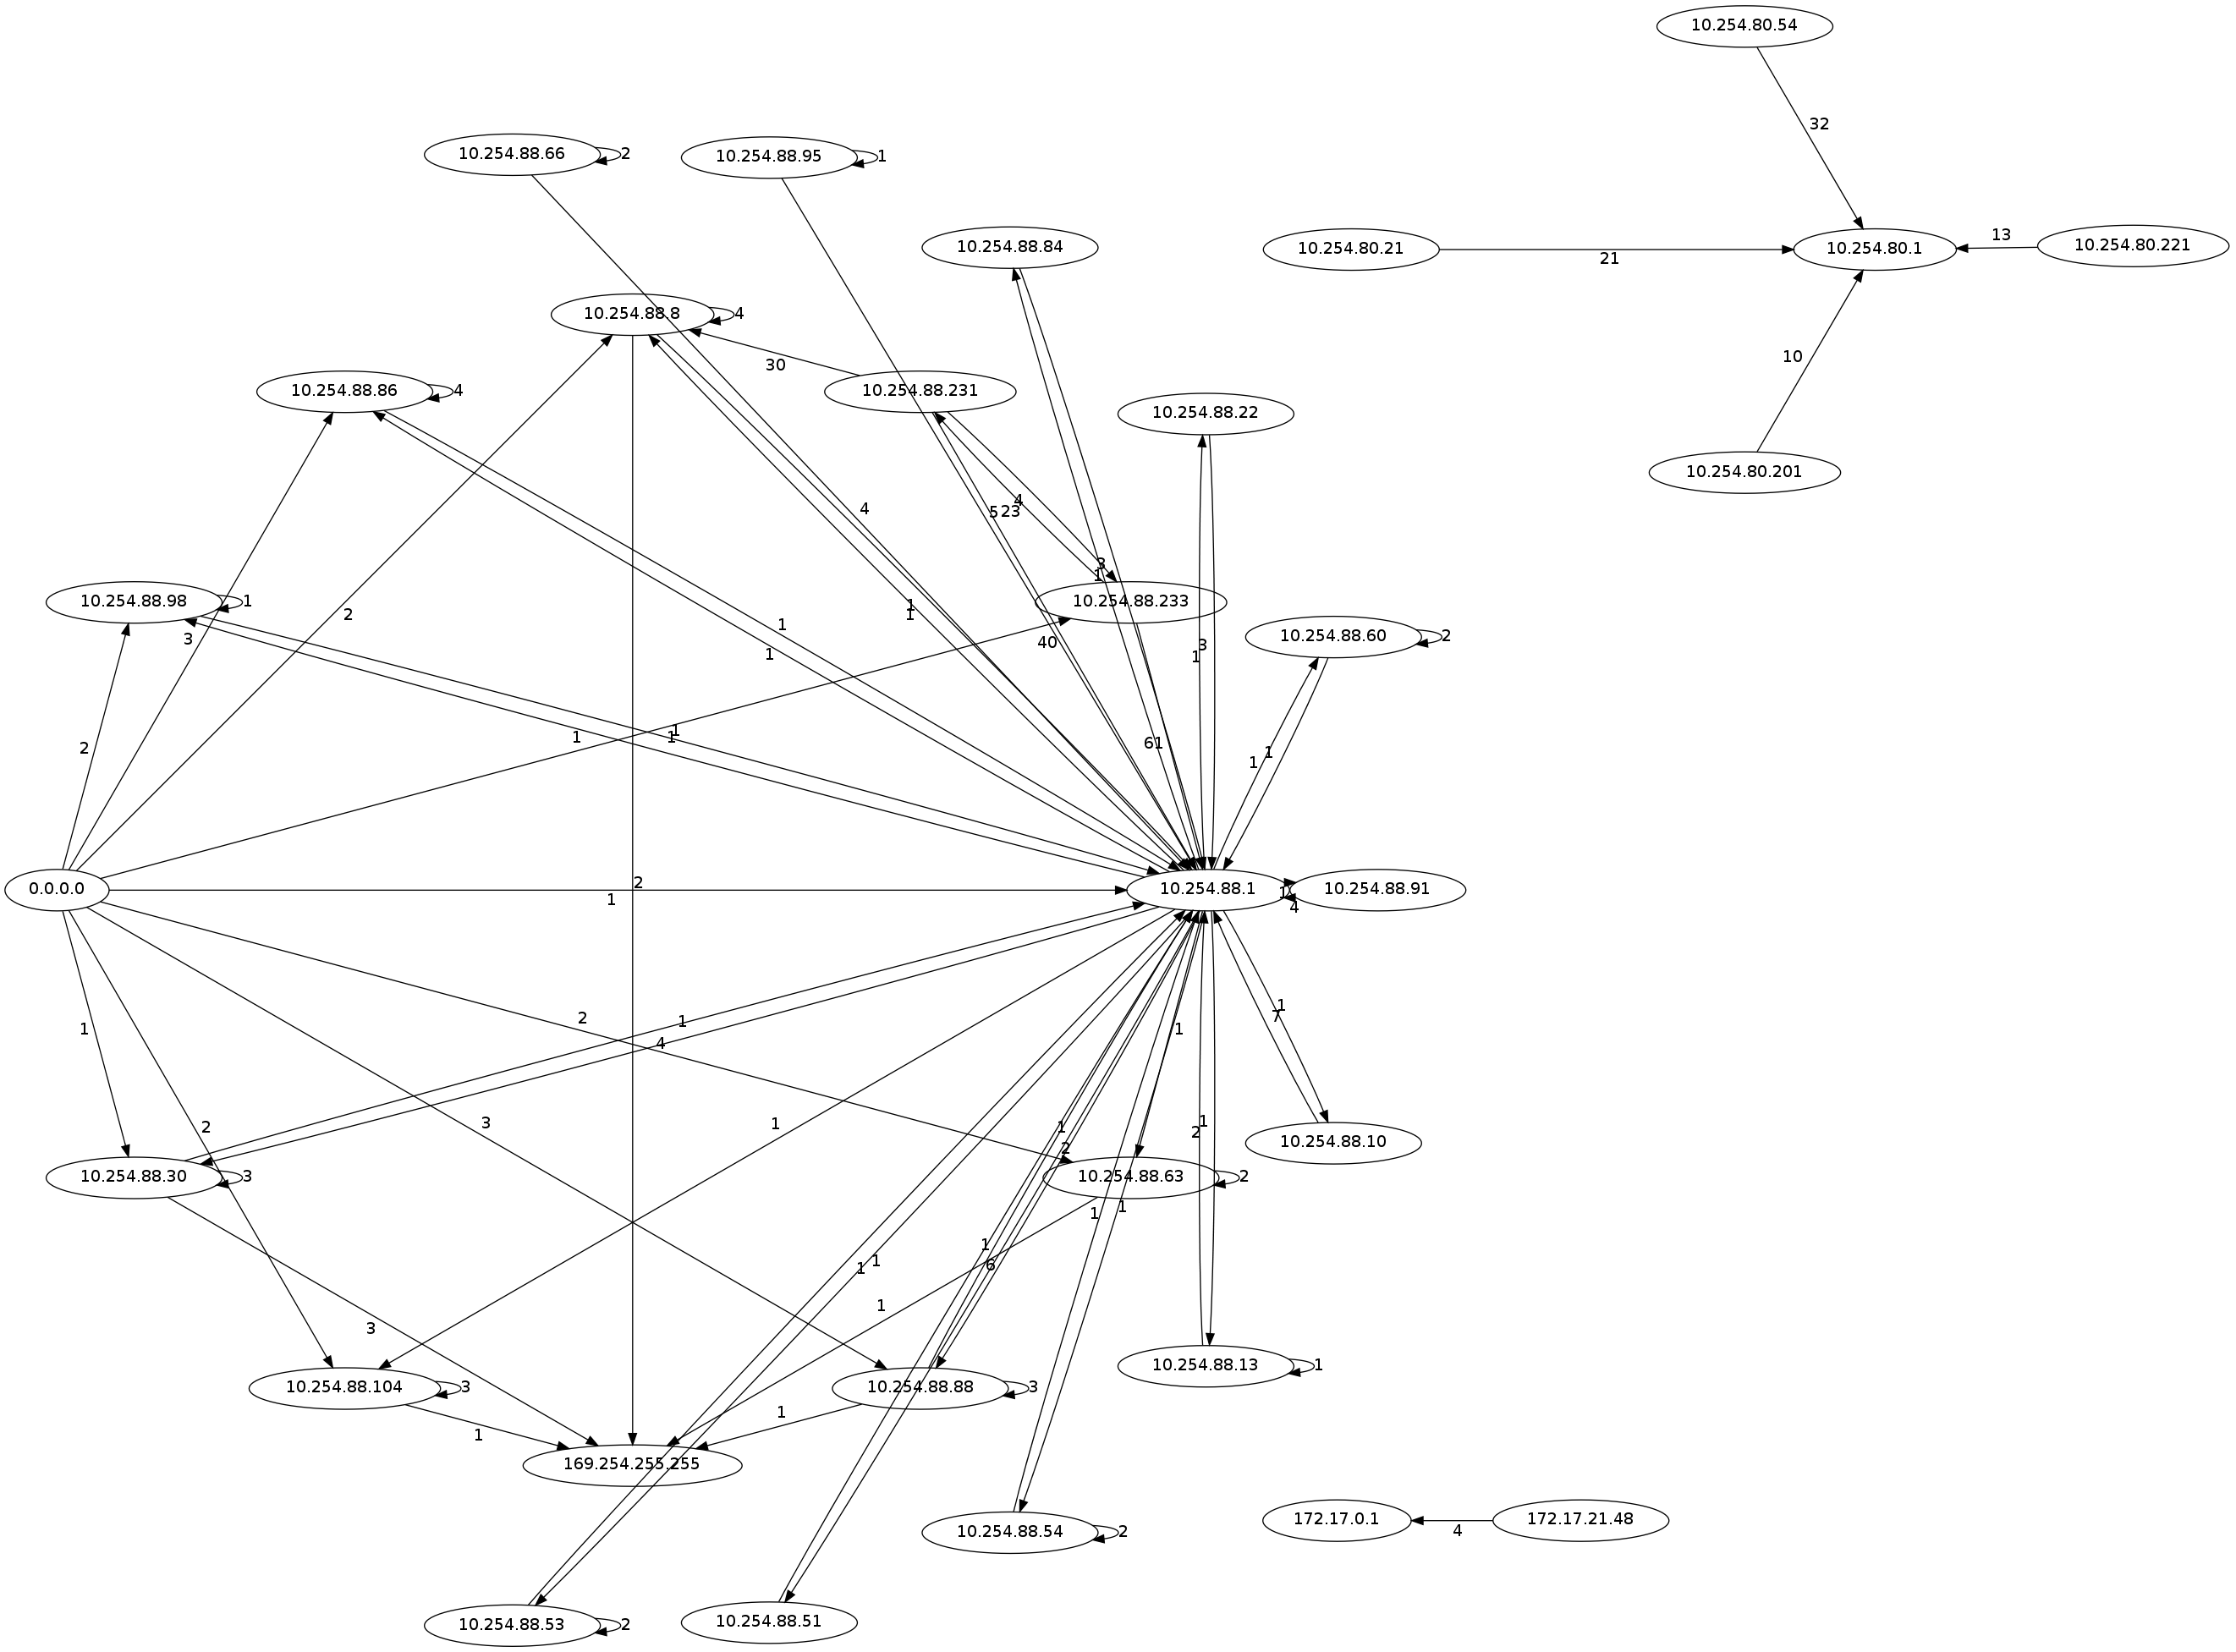
\includegraphics[width=0.9\textwidth]{resultados/starbucks/starbucks.png}
	\caption{Grafo de la red Starbucks}
\end{figure}
	

\subsection{Entrepiso}

\begin{wrapfigure}{R}{0.4\textwidth}
\vspace{-35pt}
\hspace{-35pt}
\centering
   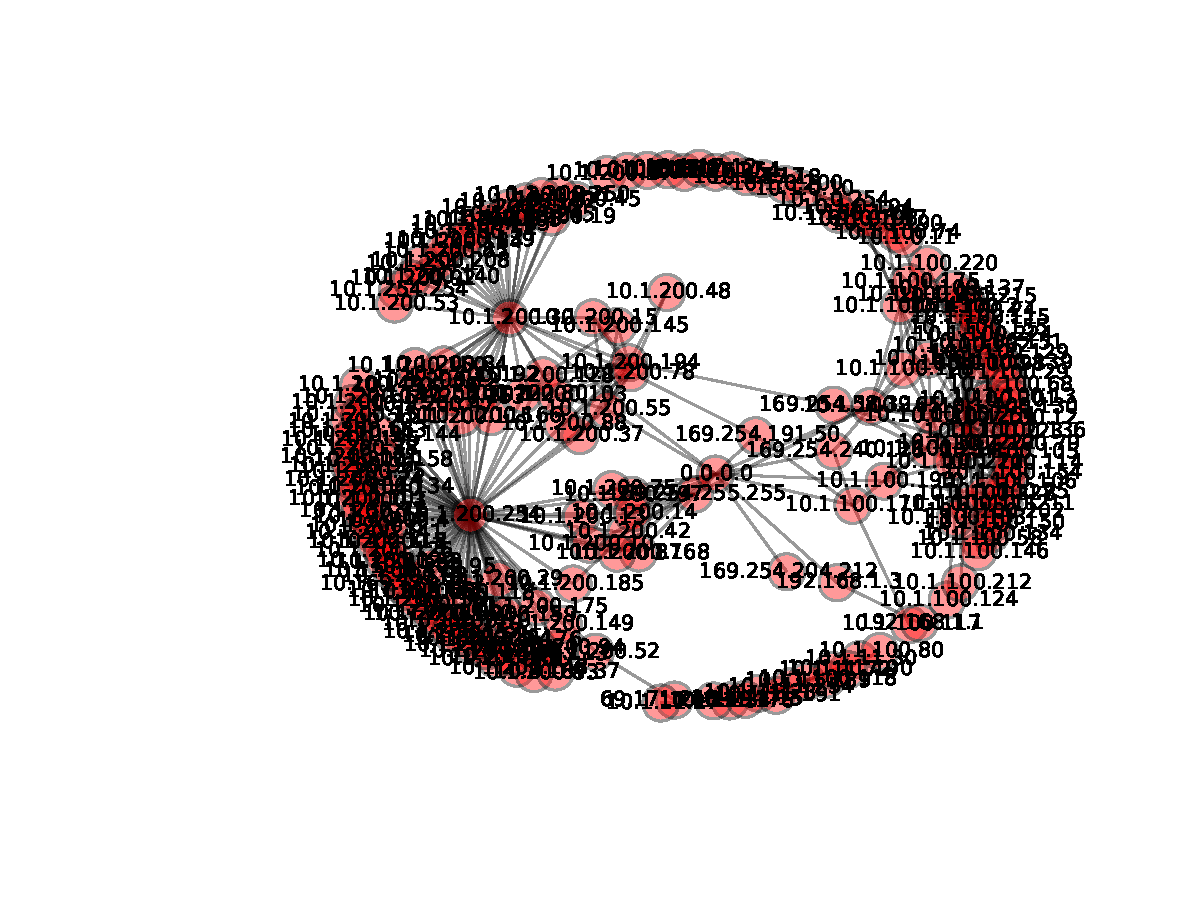
\includegraphics[width=0.4\textwidth]{resultados/entrepiso/conectividadNX.pdf}
\vspace{-30pt}
   \caption{Grafo de la red Entrepiso}
\end{wrapfigure}

En el caso del entrepiso las \emph{Figuras 8 y 10} muestran tres nodos con la forma que caracteriz\'o 
al router dentro de la casa, estos nodos son: 10.1.100.254, 10.1.200.30 y 10.1.200.254.
Sin embargo, estos poseen al menos la mitad de las aparaciones que otros nodos en 
el modelo DST, cosa que $200.30$ repite en SRC. La entrop\'ia fue: $4.25$ para el
modelo $SRC$ y $4.90$ para el modelo DST. El Entrepiso fue la red con mas entrop\'ia.
Una vez mas aparecieron direcciones sueltas, como es por ej: 10.1.11.254.

\begin{figure}[H]
	\center
	\begin{subfigure}{0.4\textwidth}
		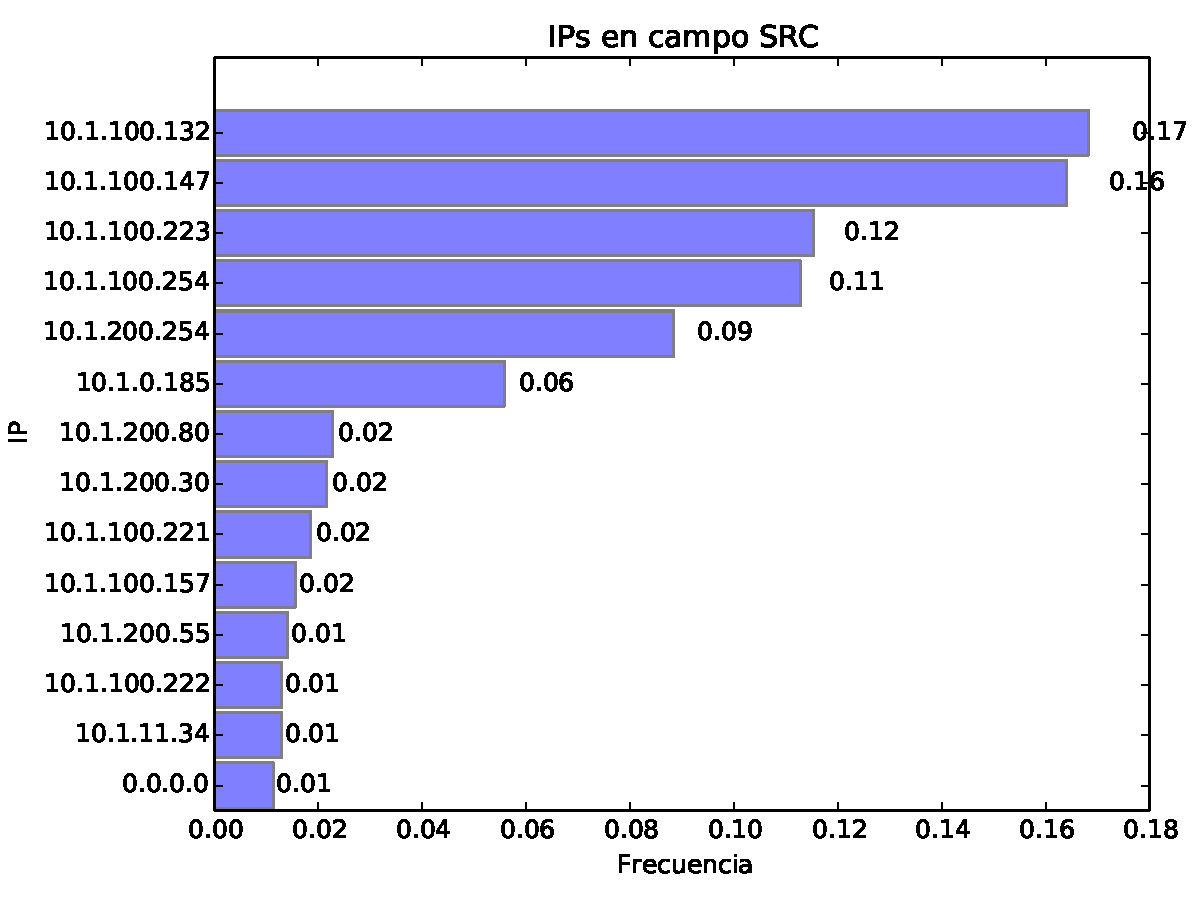
\includegraphics[width=1.0\textwidth]{resultados/entrepiso/ipsSrc_4_25991830161.pdf}
		\caption{Estimaci\'on de la probabilidad de cada s\'imbolo en modelo SRC}
	\end{subfigure}
	~
	\begin{subfigure}{0.4\textwidth}
		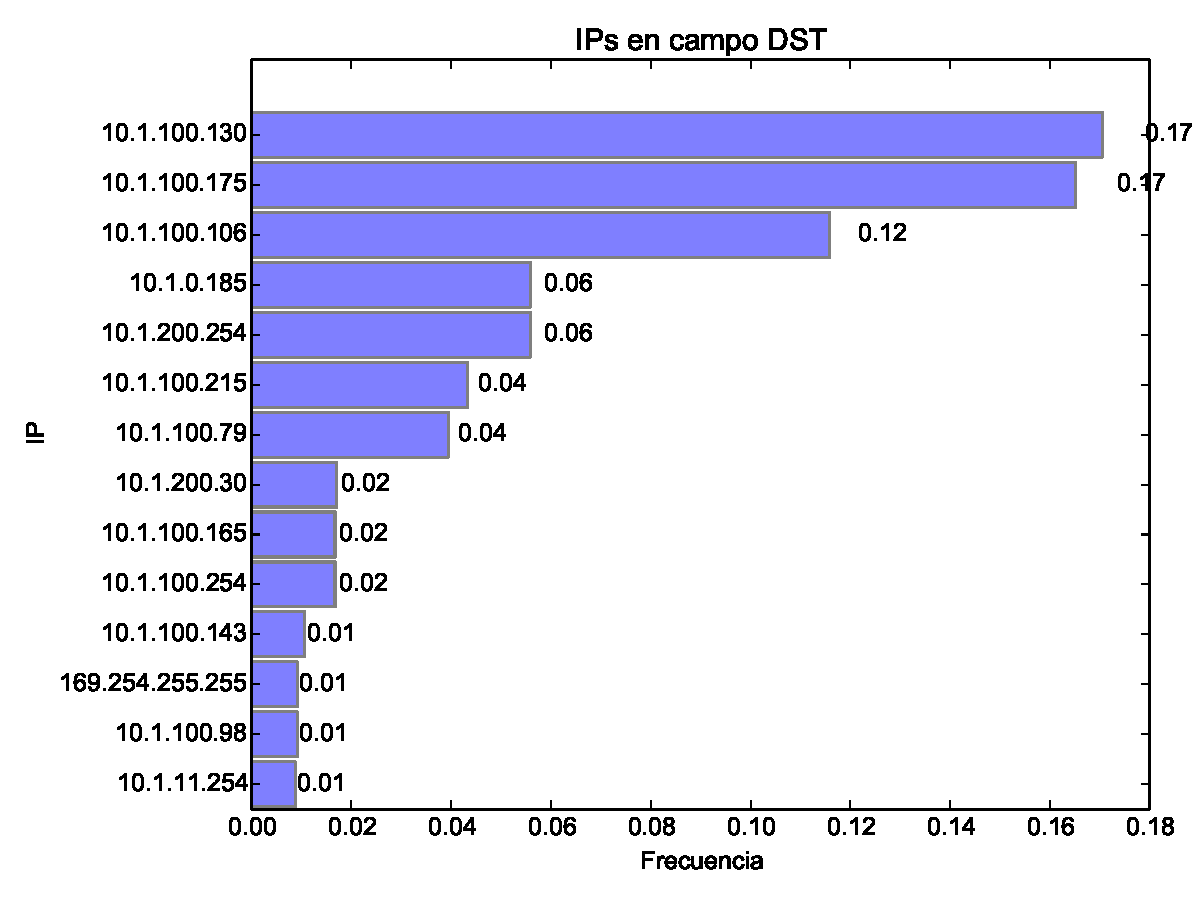
\includegraphics[width=1.0\textwidth]{resultados/entrepiso/ipsDst_4_90633854055.pdf}
		\caption{Estimaci\'on de la probabilidad de cada s\'imbolo en modelo DST}
	\end{subfigure}
\end{figure}

\begin{figure}[H]
	\includegraphics[width=1.0\textwidth]{resultados/entrepiso/conectividad.pdf}
	\caption{Digrafo de conectividad en el entrepiso}
\end{figure}


\subsection{Discusi\'on}

        En todas las redes sucedi\'o que aparecieran direcciones ip que se supone
no pertenecen a la misma. 

        En algunos casos apareci\'o la direcci\'on 169.254.255.255. Investigando
encontramos que es utilizada como broadcast por DHCP que es un protocolo de 
configuraci\'on autom\'atica de par\'ametros de red tales como direcciones IP
para interfaces y servicios.

        La direcci\'on 0.0.0.0 es el est\'andar para \emph{broadcastear} dentro
de una red local.

        Por otra parte, el resto de las direcciones IP que aparecen pueden deberse
a que los routers posean la opci\'on de \emph{Proxy ARP} habilitada, cosa que tiene 
mucho sentido en el caso del Entrepiso por ejemplo.

        A su vez, si bien en los grafos se not\'o claramente la direcci\'on ip
de los routers, \'esto s\'olo se vio reflejado en la estimaci\'on de la probabilidad
en los modelos \'unicamente en la Casa y el Starbucks. \'Esto muestra que el contar la 
cantidad de apariciones de una IP en los campos no es suficiente para detectar
los routers de la red.

        Es posible que las direcciones que aparecen con mayor frecuencia en el grafo
de pedidos ARP correspondan los dispositivos que estabam m\'as activos durante el periodo
de tiempo que se hizo el sniffing.



\section{Conclusiones}

\section{Conclusiones}

Capturando paquetes who-has de una red es posible detectar los nodos 
relevantes de una red, por ej, en todos los casos los routers resultaron
ser facilmente detectables al representar en forma de grafo los intercambios
de paquetes ARP por parte de pares de nodos, dado que los mismos son quienes
interactuan con la mayor cantidad de nodos. 

Por otra parte, el analizar la frecuencia de aparici\'on de las ips en cada
campo junto con el c\'alculo de la entrop\'ia en la red permiti\'o
demostrar emp\'iricamente que la entrop\'ia es mas baja cuando son pocos los 
s\'imbolos que aparecen
con mucha frecuencia. A su vez, vimos que de acuerdo a como modelaramos la
fuente los resultados eran distintos. Pero no solo los resultados en valores,
en los modelos SRC el router siempre ocup\'o una posici\'on
menor que en el modelo DST. 
Esto puede ser de ayuda para localizar dispositivos importantes en redes
de entrop\'ia baja, por ej, en la casa y la empresa. En redes
mas complejas como la de starbucks, no aport\'o ninguna informaci\'on mas
que demostrar que la red era ca\'otica. 


\section{Referencias}
\begin{itemize}
	\item \textbf{Computer Networks: A Systems Approach}, \textit{Larry L. Peterson and Bruce S. Davie.}
	\item \textbf{Computer Networks}, \textit{Andrew S. Tanenbaum}
	\item \textbf{Special-Purpose IP Address Registries} (RFC 6890), \textit{Internet Engineering Task Force (IETF)}
	\item \textbf{An Ethernet Address Resolution Protocol or Converting Network Protocol Addresses to 48.bit Ethernet Address for Transmission on Ethernet Hardware} (RFC 826), \textit{David C. Plummer}
\end{itemize}

\end{document}
